\chapter{Двугранные углы}\label{ch:ch4}

\begingroup
\setlength{\intextsep}{10pt plus 2pt minus 2pt}
\setlength{\textfloatsep}{12pt plus 2pt minus 2pt}

% А. П. Киселёв, «Элементарная геометрия», 23-е издание, 1914. Печатные с. 292–300.
% Страницы скана планиметрии на 11 больше печатных.
\newcommand*{\kiselevPlanimetryPage}[2]{%
    \href{https://commons.wikimedia.org/wiki/File:\%D0\%90._\%D0\%9F._\%D0\%9A\%D0\%B8\%D1\%81\%D0\%B5\%D0\%BB\%D1\%91\%D0\%B2._\%D0\%AD\%D0\%BB\%D0\%B5\%D0\%BC\%D0\%B5\%D0\%BD\%D1\%82\%D0\%B0\%D1\%80\%D0\%BD\%D0\%B0\%D1\%8F_\%D0\%B3\%D0\%B5\%D0\%BE\%D0\%BC\%D0\%B5\%D1\%82\%D1\%80\%D0\%B8\%D1\%8F_(1914).djvu?page=#1}{#2}%
}

% Печатная с. 292.
\kiselevparagraph{para:dihedral-angle-definition} \textbf{Определение.} Фигура, образованная двумя полуплоскостями \(P\) и \(Q\) (рис.~\ref{fig:kiselev-stereo-332}), исходящими из одной прямой \(AB\), вместе с частью пространства, ограниченной ими, называется \emph{двугранным углом}.

\begin{figure}[htbp]
    \centering
    \renewcommand{\thefigure}{332}
    \captionsetup{name=Рис.,labelsep=period}
    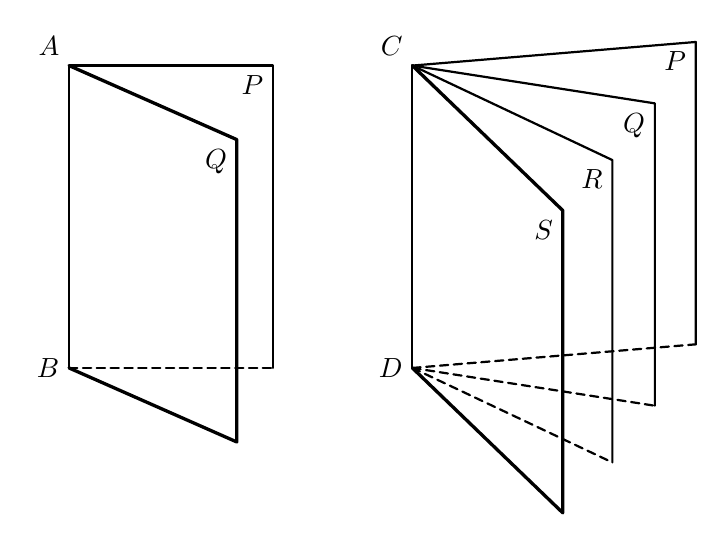
\begin{tikzpicture}[line cap=round,line join=round]
    \begin{scope}
        \coordinate (A) at (0,1.97);
        \coordinate (B) at (0,-1.87);
        \draw[thick] (B) -- (A) -- (2.59,1.97) -- (2.59,-1.87);
        \draw[thick,densely dashed] (B) -- (2.59,-1.87);
        \draw[very thick] (A) -- (2.13,1.03) -- (2.13,-2.81) -- (B);
        \node[above left] at (A) {\(A\)};
        \node[left] at (B) {\(B\)};
        \node[below left] at (2.59,1.97) {\(P\)};
        \node[below left] at (2.13,1.03) {\(Q\)};
    \end{scope}
    \begin{scope}[xshift=4.36cm]
        \coordinate (C) at (0,1.97);
        \coordinate (D) at (0,-1.87);
        \draw[thick] (D) -- (C);
        \foreach \x/\top/\bottom/\face in {3.6/2.27/-1.57/P,3.08/1.49/-2.35/Q,2.54/0.77/-3.07/R}{
            \draw[thick] (C) -- (\x,\top) -- (\x,\bottom);
            \draw[thick,densely dashed] (D) -- (\x,\bottom);
            \node[below left] at (\x,\top) {\(\face\)};
        }
        \draw[very thick] (C) -- (1.91,0.13) -- (1.91,-3.71) -- (D);
        \node[below left] at (1.91,0.13) {\(S\)};
        \node[above left] at (C) {\(C\)};
        \node[left] at (D) {\(D\)};
    \end{scope}
\end{tikzpicture}

    \caption{Двугранные углы с рёбрами \(AB\) и \(CD\)}\label{fig:kiselev-stereo-332}
\end{figure}

Прямая \(AB\) называется \emph{ребром}, а полуплоскости \(P\) и \(Q\) --- сторонами, или \emph{гранями}, двугранного угла. Такой угол обычно обозначают двумя буквами, поставленными у его ребра (двугранный угол \(AB\)).
% Печатная с. 293.
Но если при одном ребре лежат несколько двугранных углов, то каждый из них обозначают четырьмя буквами, из которых две средние стоят при ребре, а две крайние --- у граней (например, двугранный угол \(SCDR\)).

Если через ребро \(CD\) двугранного угла \(PCDS\) (рис.~\ref{fig:kiselev-stereo-332}) проведём внутри него, то есть в той части пространства, которая принадлежит углу, какие-нибудь полуплоскости \(R,Q,\ldots\), то образовавшиеся при этом двугранные углы \(RCDS,QCDR,\ldots\) рассматриваются как части первого двугранного угла.

Если из произвольной точки \(D\) ребра \(AB\) (рис.~\ref{fig:kiselev-stereo-333}) проведём на каждой грани по перпендикуляру к ребру, то образованный ими угол \(CDE\) называется \emph{линейным углом двугранного угла}. Величина линейного угла не зависит от положения точки \(D\) на ребре. Так, линейные углы \(CDE\) и \(C_1D_1E_1\) равны, потому что их стороны соответственно параллельны и одинаково направлены.

\begin{figure}[htbp]
    \centering
    \renewcommand{\thefigure}{333}
    \captionsetup{name=Рис.,labelsep=period}
    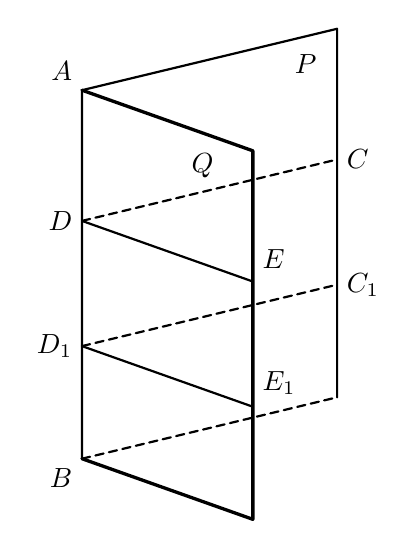
\begin{tikzpicture}[line cap=round,line join=round]
    \coordinate (A) at (0,2.55);
    \coordinate (B) at (0,-2.13);
    \coordinate (D) at (0,0.89);
    \coordinate (D1) at (0,-0.7);
    \coordinate (C) at (3.24,1.67);
    \coordinate (C1) at (3.24,0.08);
    \coordinate (E) at (2.17,0.12);
    \coordinate (E1) at (2.17,-1.47);

    \draw[thick] (B) -- (A) -- (3.24,3.33) -- (3.24,-1.35);
    \draw[thick,densely dashed] (B) -- (3.24,-1.35) (D) -- (C) (D1) -- (C1);
    \draw[very thick] (A) -- (2.17,1.78) -- (2.17,-2.90) -- (B);
    \draw[thick] (D) -- (E) (D1) -- (E1);
    \node[above left] at (A) {\(A\)};
    \node[below left] at (B) {\(B\)};
    \node[left] at (D) {\(D\)};
    \node[left] at (D1) {\(D_1\)};
    \node[right] at (C) {\(C\)};
    \node[right] at (C1) {\(C_1\)};
    \node[above right,yshift=1pt] at (E) {\(E\)};
    \node[above right,yshift=1pt] at (E1) {\(E_1\)};
    \node at (2.84,2.88) {\(P\)};
    \node at (1.53,1.59) {\(Q\)};
\end{tikzpicture}

    \caption{Линейные углы \(CDE\) и \(C_1D_1E_1\) двугранного угла}\label{fig:kiselev-stereo-333}
\end{figure}

Плоскость линейного угла перпендикулярна к ребру, так как она содержит две прямые, перпендикулярные к нему (\hyperref[para:perpendicular-plane-criterion]{см.~§~\ref*{para:perpendicular-plane-criterion}}).

\kiselevparagraph{para:dihedral-angles-comparison} \textbf{Равенство и неравенство двугранных углов.} Два двугранных угла считаются \emph{равными}, если при наложении они могут совместиться. В противном случае тот из углов считается меньшим, который может составить часть другого угла.

Можно рассматривать \emph{сумму, разность, произведение и частное двугранных углов} в том же смысле, что и для углов планиметрии. Подобно этим углам, двугранные углы могут быть \emph{смежными, прямыми, вертикальными} и т.~д.

\kiselevparagraph{para:dihedral-and-linear-angle-comparison} \textbf{Теоремы.}

\begin{enumerate}[label=\arabic*),ref=\arabic*]
    \item \textbf{Равным двугранным углам соответствуют равные линейные углы.}
    \item \textbf{Большему двугранному углу соответствует больший линейный угол.}
\end{enumerate}

% Печатная с. 294.
Пусть \(PABQ\) и \(P_1A_1B_1Q_1\) (рис.~\ref{fig:kiselev-stereo-334}) будут два двугранных угла. Наложим угол \(A_1B_1\) на угол \(AB\) так, чтобы ребро \(A_1B_1\) совпало с ребром \(AB\), а грань \(P_1\) --- с гранью \(P\). Тогда, если эти двугранные углы равны, грань \(Q_1\) совпадёт с \(Q\). Если же двугранные углы не равны, грань \(Q_1\) не совпадёт с \(Q\). Например, она займёт положение \(Q_{11}\), если угол \(A_1B_1\) меньше угла \(AB\).

\begin{figure}[htbp]
    \centering
    \renewcommand{\thefigure}{334}
    \captionsetup{name=Рис.,labelsep=period}
    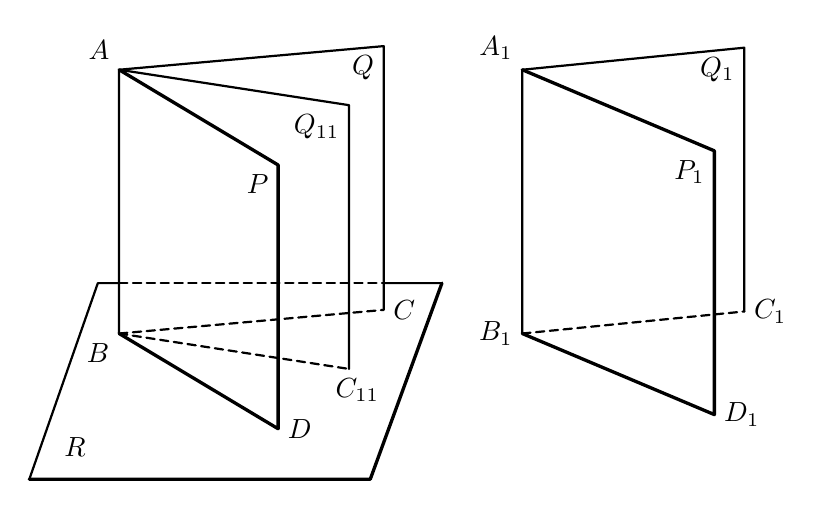
\begin{tikzpicture}[line cap=round,line join=round]
    \coordinate (A) at (0,2.45);
    \coordinate (B) at (0,-0.9);
    \coordinate (C) at (3.36,-0.6);
    \coordinate (C11) at (2.92,-1.35);
    \coordinate (D) at (2.02,-2.11);
    \draw[thick] (-1.14,-2.75) -- (-0.27,-0.26) -- (0,-0.26)
        (3.36,-0.26) -- (4.10,-0.26);
    \draw[thick,densely dashed] (0,-0.26) -- (3.36,-0.26);
    \draw[very thick] (-1.14,-2.75) -- (3.19,-2.75) -- (4.10,-0.26);
    \draw[thick] (B) -- (A) -- (3.36,2.75) -- (C)
        (A) -- (2.92,2.00) -- (C11);
    \draw[thick,densely dashed] (B) -- (C) (B) -- (C11);
    \draw[very thick] (A) -- (2.02,1.24) -- (D) -- (B);
    \node[above left] at (A) {\(A\)};
    \node[below left] at (B) {\(B\)};
    \node[right] at (C) {\(C\)};
    \node[below,xshift=3pt] at (C11) {\(C_{11}\)};
    \node[right] at (D) {\(D\)};
    \node[below left] at (3.36,2.75) {\(Q\)};
    \node[below left] at (2.92,2.00) {\(Q_{11}\)};
    \node[below left] at (2.02,1.24) {\(P\)};
    \node at (-0.56,-2.34) {\(R\)};

    \begin{scope}[xshift=5.12cm]
        \coordinate (A1) at (0,2.45);
        \coordinate (B1) at (0,-0.9);
        \coordinate (C1) at (2.82,-0.62);
        \coordinate (D1) at (2.44,-1.93);
        \draw[thick] (B1) -- (A1) -- (2.82,2.73) -- (C1);
        \draw[thick,densely dashed] (B1) -- (C1);
        \draw[very thick] (A1) -- (2.44,1.42) -- (D1) -- (B1);
        \node[above left] at (A1) {\(A_1\)};
        \node[left] at (B1) {\(B_1\)};
        \node[right] at (C1) {\(C_1\)};
        \node[right] at (D1) {\(D_1\)};
        \node[below left] at (2.82,2.73) {\(Q_1\)};
        \node[below left] at (2.44,1.42) {\(P_1\)};
    \end{scope}
\end{tikzpicture}

    \caption{Наложение двугранных углов \(PABQ\) и \(P_1A_1B_1Q_1\)}\label{fig:kiselev-stereo-334}
\end{figure}

Заметив это, возьмём на общем ребре какую-нибудь точку \(B\) и проведём через неё плоскость \(R\), перпендикулярную к ребру. От пересечения этой плоскости с гранями двугранных углов получатся линейные углы. Ясно, что если двугранные углы совпадут, то у них окажется один и тот же линейный угол, а именно \(CBD\). Если же двугранные углы не совпадут, например, если грань \(Q_1\) займёт положение \(Q_{11}\), то у большего двугранного угла окажется больший линейный угол, а именно \(CBD>C_{11}BD\).

\needspace{3\baselineskip}
\kiselevparagraph{para:linear-and-dihedral-angle-comparison} \textbf{Обратные теоремы.}

\begin{enumerate}[label=\arabic*),ref=\arabic*]
    \item \textbf{Равным линейным углам соответствуют равные двугранные углы.}
    \item \textbf{Большему линейному углу соответствует больший двугранный угол.}
\end{enumerate}

Эти теоремы легко доказываются от противного (\kiselevPlanimetryPage{46}{см.~Планиметрия, §~51}).

\kiselevparagraph{para:superposition-of-spatial-figures} \textbf{Замечание.} Мы принимаем за очевидное, что \emph{наложение одной фигуры на другую}, часто употребляемое в стереометрии, всегда можно выполнить в такой последовательности:

\begin{enumerate}[label=\arabic*),ref=\arabic*]
    % Печатная с. 295 начинается со слова «фигур» в пункте 1.
    \item совмещаем какие-нибудь две точки фигур;
    \item совмещаем какие-нибудь две полупрямые, исходящие из совпавших точек;
    \item совмещаем какие-нибудь две полуплоскости, исходящие из совпавших прямых.
\end{enumerate}

Совместятся ли при этом другие элементы фигур, зависит от их свойств.

\kiselevparagraph{para:right-and-equal-dihedral-angles} \textbf{Следствия.}

\begin{enumerate}[label=\arabic*),ref=\arabic*]
    \item\label{item:right-dihedral-and-linear-angle} \textbf{Прямому двугранному углу соответствует прямой линейный угол и обратно.}

    Пусть двугранный угол \(PABQ\) (рис.~\ref{fig:kiselev-stereo-335}) прямой. Это значит, что он равен смежному углу \(QABP_1\). Но в таком случае линейные углы \(CDE\) и \(CDE_1\) также равны. А так как они смежные, то каждый из них должен быть прямым. Обратно, если равны смежные линейные углы \(CDE\) и \(CDE_1\), то равны и смежные двугранные углы, то есть каждый из них должен быть прямым.

    \item \textbf{Прямые двугранные углы равны}, потому что у них равны линейные углы. По той же причине:
    \item \textbf{вертикальные двугранные углы равны;}
    \item \textbf{двугранные углы с соответственно параллельными и одинаково направленными гранями равны.}
\end{enumerate}

\begin{figure}[htbp]
    \centering
    \renewcommand{\thefigure}{335}
    \captionsetup{name=Рис.,labelsep=period}
    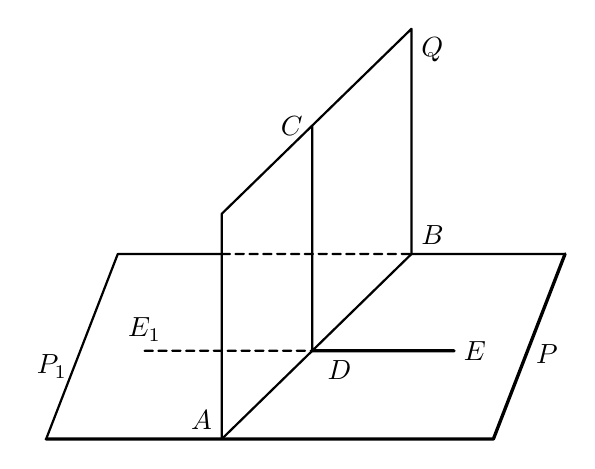
\begin{tikzpicture}[line cap=round,line join=round]
    \coordinate (A) at (-0.97,-1.3);
    \coordinate (B) at (1.44,1.05);
    \path (A) -- (B) coordinate[pos=0.477] (D);
    \coordinate (C) at (0.18,2.68);
    \draw[thick] (-3.20,-1.3) -- (-2.29,1.05) -- (-0.97,1.05)
        (1.44,1.05) -- (3.39,1.05);
    \draw[thick,densely dashed] (-0.97,1.05) -- (B)
        (-1.95,-0.18) -- (D);
    \draw[very thick] (-3.20,-1.3) -- (2.48,-1.3) -- (3.39,1.05);
    \draw[thick] (A) -- (-0.97,1.56) -- (1.44,3.91) -- (B) -- (A)
        (D) -- (C);
    \draw[very thick] (D) -- (1.98,-0.18);
    \node[above left] at (A) {\(A\)};
    \node[above right] at (B) {\(B\)};
    \node[left] at (C) {\(C\)};
    \node[below right,xshift=2pt] at (D) {\(D\)};
    \node[right] at (1.98,-0.18) {\(E\)};
    \node[above] at (-1.95,-0.18) {\(E_1\)};
    \node[right] at (1.44,3.64) {\(Q\)};
    \node[right] at (2.9,-0.22) {\(P\)};
    \node[left] at (-2.81,-0.38) {\(P_1\)};
\end{tikzpicture}

    \caption{Прямой двугранный угол и его линейный угол}\label{fig:kiselev-stereo-335}
\end{figure}

\kiselevparagraph{para:ratio-of-dihedral-angles} \textbf{Теорема. Двугранные углы относятся, как их линейные углы.}

При доказательстве рассмотрим отдельно два случая:

\begin{figure}[htbp]
    \centering
    \renewcommand{\thefigure}{336}
    \captionsetup{name=Рис.,labelsep=period}
    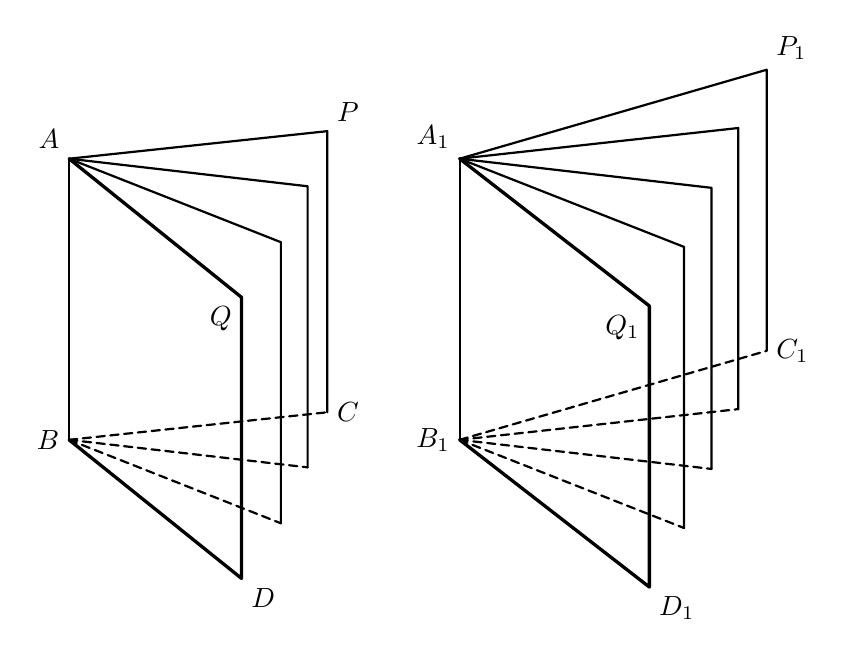
\begin{tikzpicture}[line cap=round,line join=round]
    \begin{scope}
        \coordinate (A) at (0,2.08);
        \coordinate (B) at (0,-1.49);
        \draw[thick] (A) -- (B);
        % Три части угла AB.
        \foreach \x/\top/\bottom in {3.28/2.43/-1.14,3.03/1.73/-1.84,2.69/1.02/-2.55}{
            \draw[thick] (A) -- (\x,\top) -- (\x,\bottom);
            \draw[thick,densely dashed] (B) -- (\x,\bottom);
        }
        \draw[very thick] (A) -- (2.19,0.32) -- (2.19,-3.25) -- (B);
        \node[above left] at (A) {\(A\)};
        \node[left] at (B) {\(B\)};
        \node[right] at (3.28,-1.14) {\(C\)};
        \node[below right] at (2.19,-3.25) {\(D\)};
        \node[above right] at (3.28,2.43) {\(P\)};
        \node[below left] at (2.19,0.32) {\(Q\)};
    \end{scope}
    \begin{scope}[xshift=4.96cm]
        \coordinate (A1) at (0,2.08);
        \coordinate (B1) at (0,-1.49);
        \draw[thick] (A1) -- (B1);
        % Четыре части угла A1B1.
        \foreach \x/\top/\bottom in {3.9/3.21/-0.36,3.54/2.47/-1.10,3.20/1.71/-1.86,2.85/0.96/-2.61}{
            \draw[thick] (A1) -- (\x,\top) -- (\x,\bottom);
            \draw[thick,densely dashed] (B1) -- (\x,\bottom);
        }
        \draw[very thick] (A1) -- (2.41,0.21) -- (2.41,-3.36) -- (B1);
        \node[above left] at (A1) {\(A_1\)};
        \node[left] at (B1) {\(B_1\)};
        \node[right] at (3.9,-0.36) {\(C_1\)};
        \node[below right] at (2.41,-3.36) {\(D_1\)};
        \node[above right] at (3.9,3.21) {\(P_1\)};
        \node[below left] at (2.41,0.21) {\(Q_1\)};
    \end{scope}
\end{tikzpicture}

    \caption{Деление двугранных углов на равные части}\label{fig:kiselev-stereo-336}
\end{figure}

\begin{enumerate}[label=\arabic*),ref=\arabic*]
    \item \emph{Линейные углы \(CBD\) и \(C_1B_1D_1\) соизмеримы} (рис.~\ref{fig:kiselev-stereo-336}). Пусть их общая мера содержится в первом угле \(m\) раз, а во втором \(n\) раз. Проведём ряд плоскостей через рёбра и прямые, делящие линейные углы на части, равные общей мере. Тогда мы разделим угол \(AB\) на \(m\), а угол \(A_1B_1\) на
    % Печатная с. 296.
    \(n\) частей, которые все равны между собой вследствие равенства линейных углов. Поэтому
    \[
        \frac{\angle CBD}{\angle C_1B_1D_1}=\frac{m}{n}
        \quad\text{и}\quad
        \frac{\text{дв. уг. } AB}{\text{дв. уг. } A_1B_1}=\frac{m}{n}.
    \]
    Откуда
    \[
        \frac{\text{дв. уг. } AB}{\text{дв. уг. } A_1B_1}=
        \frac{\angle CBD}{\angle C_1B_1D_1}.
    \]

    \item \emph{Линейные углы несоизмеримы.} Разделим (рис.~\ref{fig:kiselev-stereo-336}) угол \(C_1B_1D_1\) на \(n\) равных частей. Пусть \(1/n\) этого угла содержится в угле \(CBD\) больше \(m\), но меньше \(m+1\) раз. Тогда приближённое отношение углов \(CBD\) и \(C_1B_1D_1\) с точностью до \(1/n\) (с недостатком) равно \(m/n\). Проведя плоскости так же, как и в первом случае, найдём, что приближённое отношение двугранных углов \(AB\) и \(A_1B_1\) с точностью до \(1/n\) (с недостатком) также равно \(m/n\). Таким образом, приближённые отношения равны при любом \(n\), а в этом случае мы условились считать несоизмеримые отношения \emph{равными}.
\end{enumerate}

\kiselevparagraph{para:measure-of-dihedral-angle} \textbf{Следствие.} Если за единицу измерения двугранных углов возьмём такой угол, который соответствует единице измерения линейных углов, то можно сказать, что \emph{двугранный угол измеряется его линейным углом}.


\section*{Перпендикулярные плоскости}
\addcontentsline{toc}{section}{Перпендикулярные плоскости}

\kiselevparagraph{para:perpendicular-planes-definition} \textbf{Определение.} Две плоскости называются \emph{взаимно перпендикулярными}, если, пересекаясь, они образуют \emph{прямые двугранные углы}. Возможность существования таких плоскостей показывает следующая теорема, указывающая \emph{признак перпендикулярности двух плоскостей}.

\kiselevparagraph{para:perpendicular-planes-criterion} \textbf{Теорема. Если плоскость} \(P\) (рис.~\ref{fig:kiselev-stereo-337}) \textbf{проходит через перпендикуляр} \(AB\) \textbf{к другой плоскости} \(Q\)\textbf{, то она перпендикулярна к этой плоскости.}

\begin{figure}[htbp]
    \centering
    \renewcommand{\thefigure}{337}
    \captionsetup{name=Рис.,labelsep=period}
    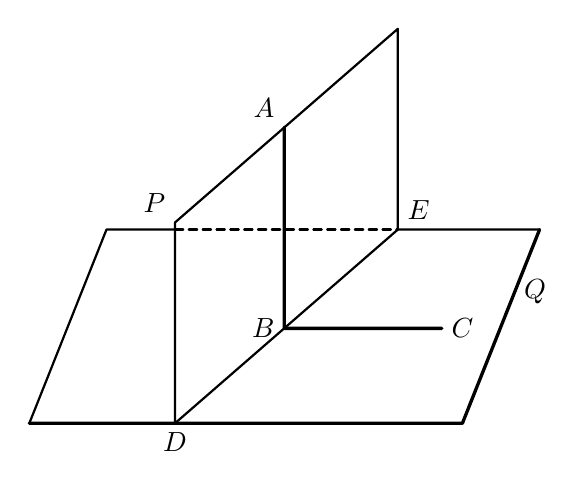
\begin{tikzpicture}[line cap=round,line join=round]
    \coordinate (D) at (-1.42,-1.38);
    \coordinate (E) at (1.41,1.08);
    \path (D) -- (E) coordinate[pos=0.49] (B);
    \coordinate (A) at (-0.033,2.38);
    \coordinate (C) at (1.97,-0.175);
    \draw[thick] (-3.27,-1.38) -- (-2.29,1.08) -- (-1.42,1.08)
        (E) -- (3.21,1.08);
    \draw[thick,densely dashed] (-1.42,1.08) -- (E);
    \draw[very thick] (-3.27,-1.38) -- (2.23,-1.38) -- (3.21,1.08);
    \draw[thick] (D) -- (-1.42,1.17) -- (1.41,3.63) -- (E) -- (D);
    \draw[very thick] (A) -- (B) -- (C);
    \node[above left] at (A) {\(A\)};
    \node[left] at (B) {\(B\)};
    \node[right] at (C) {\(C\)};
    \node[below] at (D) {\(D\)};
    \node[above right] at (E) {\(E\)};
    \node[above left] at (-1.42,1.17) {\(P\)};
    \node[right] at (2.89,0.29) {\(Q\)};
\end{tikzpicture}

    \caption{Плоскость \(P\) проходит через перпендикуляр \(AB\) к плоскости \(Q\)}\label{fig:kiselev-stereo-337}
\end{figure}

% Печатная с. 297.
В плоскости \(Q\) проведём \(BC\perp DE\). Тогда угол \(ABC\) будет линейным углом двугранного угла \(PDEQ\). Так как прямая \(AB\), по условию, перпендикулярна к \(Q\), то \(AB\perp BC\). Значит, угол \(ABC\) прямой, а потому и двугранный угол прямой (\hyperref[item:right-dihedral-and-linear-angle]{см.~§~\ref*{para:right-and-equal-dihedral-angles}, пункт~\ref*{item:right-dihedral-and-linear-angle}}), то есть плоскость \(P\) перпендикулярна к \(Q\).

Следующие две теоремы выражают \emph{главные свойства перпендикулярных плоскостей}.

\kiselevparagraph{para:normal-in-perpendicular-plane} \textbf{Теорема. Если две плоскости} \(P\) и \(Q\) (рис.~\ref{fig:kiselev-stereo-338}) \textbf{взаимно перпендикулярны и к одной из них} (к \(Q\)) \textbf{проведён перпендикуляр} \(AB\)\textbf{, имеющий общую точку} \(A\) \textbf{с другой плоскостью} (с \(P\))\textbf{, то он весь лежит в этой плоскости.}

\begin{figure}[htbp]
    \centering
    \renewcommand{\thefigure}{338}
    \captionsetup{name=Рис.,labelsep=period}
    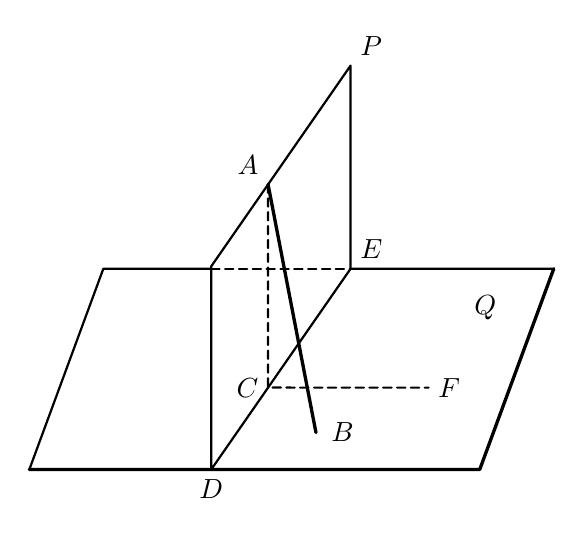
\begin{tikzpicture}[line cap=round,line join=round]
    \coordinate (D) at (-0.81,-1.50);
    \coordinate (E) at (0.96,1.05);
    \path (D) -- (E) coordinate[pos=0.408] (C);
    \coordinate (A) at (-0.088,2.12);
    \coordinate (B) at (0.52,-1.03);
    \coordinate (F) at (1.95,-0.46);
    \draw[thick] (-3.12,-1.50) -- (-2.18,1.05) -- (-0.81,1.05)
        (E) -- (3.54,1.05);
    \draw[thick,densely dashed] (-0.81,1.05) -- (E);
    \draw[very thick] (-3.12,-1.50) -- (2.60,-1.50) -- (3.54,1.05);
    \draw[thick] (D) -- (-0.81,1.08) -- (0.96,3.63) -- (E) -- (D);
    \draw[very thick] (A) -- (B);
    \draw[thick,densely dashed] (A) -- (C) -- (F);
    \node[above left] at (A) {\(A\)};
    \node[right,xshift=2pt] at (B) {\(B\)};
    \node[left] at (C) {\(C\)};
    \node[below] at (D) {\(D\)};
    \node[above right] at (E) {\(E\)};
    \node[right] at (F) {\(F\)};
    \node[above right] at (0.96,3.63) {\(P\)};
    \node at (2.67,0.55) {\(Q\)};
\end{tikzpicture}

    \caption{Предположение, что \(AB\) не лежит в плоскости \(P\)}\label{fig:kiselev-stereo-338}
\end{figure}

Предположим, что \(AB\) не лежит в плоскости \(P\), как изображено на рисунке. Проведём в этой плоскости \(AC\perp DE\), а в плоскости \(Q\) проведём \(CF\perp DE\). Тогда угол \(ACF\), как линейный угол прямого двугранного угла, будет прямым. Поэтому прямая \(AC\), образуя прямые углы с \(DE\) и \(CF\), будет перпендикуляром к плоскости \(Q\). У нас тогда будет два перпендикуляра, опущенных из одной и той же точки \(A\) на плоскость \(Q\), именно \(AB\) и \(AC\). Так как это невозможно, то нельзя допустить, чтобы перпендикуляр \(AB\) не лежал в плоскости \(P\).

\kiselevparagraph{para:intersection-normal-to-third-plane} \textbf{Следствие. Пересечение} \(AB\) (рис.~\ref{fig:kiselev-stereo-339}) \textbf{двух плоскостей} \(P\) и \(Q\)\textbf{, перпендикулярных к третьей плоскости} \(R\)\textbf{, есть перпендикуляр к этой плоскости.}

\begin{figure}[htbp]
    \centering
    \renewcommand{\thefigure}{339}
    \captionsetup{name=Рис.,labelsep=period}
    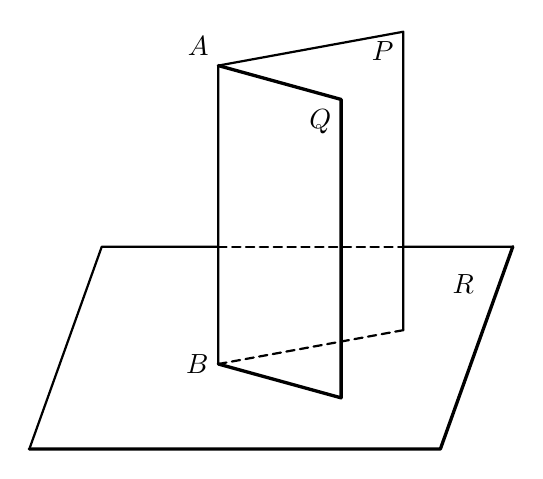
\begin{tikzpicture}[line cap=round,line join=round]
    \coordinate (A) at (-0.60,3.29);
    \coordinate (B) at (-0.60,-0.50);
    \draw[thick] (-3.0,-1.58) -- (-2.08,0.99) -- (-0.60,0.99)
        (1.75,0.99) -- (3.14,0.99);
    \draw[thick,densely dashed] (-0.60,0.99) -- (1.75,0.99);
    \draw[very thick] (-3.0,-1.58) -- (2.22,-1.58) -- (3.14,0.99);
    \draw[thick] (B) -- (A) -- (1.75,3.72) -- (1.75,-0.07);
    \draw[thick,densely dashed] (B) -- (1.75,-0.07);
    \draw[very thick] (A) -- (0.96,2.86) -- (0.96,-0.93) -- (B);
    \node[above left] at (A) {\(A\)};
    \node[left] at (B) {\(B\)};
    \node[below left] at (1.75,3.72) {\(P\)};
    \node[below left] at (0.96,2.86) {\(Q\)};
    \node at (2.51,0.51) {\(R\)};
\end{tikzpicture}

    \caption{Линия пересечения \(AB\) перпендикулярна к плоскости \(R\)}\label{fig:kiselev-stereo-339}
\end{figure}

% Доказательство продолжается на печатной с. 298.
Действительно, если через какую-нибудь точку \(A\) линии пересечения проведём перпендикуляр к плоскости \(R\), то этот перпендикуляр, согласно \hyperref[para:normal-in-perpendicular-plane]{предыдущей теореме}, должен лежать и в плоскости \(Q\), и в плоскости \(P\). Значит, он сольётся с \(AB\).

\section*{Угол двух скрещивающихся прямых}
\addcontentsline{toc}{section}{Угол двух скрещивающихся прямых}

\kiselevparagraph{para:angle-between-skew-lines} Мы видели (\hyperref[para:skew-and-parallel-lines]{см.~§~\ref*{para:skew-and-parallel-lines}}), что в пространстве можно взять такие прямые, которые не пересекаются и в то же время не параллельны, так как не лежат в одной плоскости. Для таких \emph{скрещивающихся} прямых дадим следующее определение.

\textbf{Определение.} \emph{Углом двух скрещивающихся прямых} \(AB\) и \(CD\) (рис.~\ref{fig:kiselev-stereo-340}), положение и направление которых заданы, называется угол \(MON\), который получится, если из произвольной точки пространства \(O\) проведём полупрямые \(OM\) и \(ON\), \emph{соответственно параллельные данным прямым} \(AB\) и \(CD\) \emph{и одинаково с ними направленные}.

\begin{figure}[htbp]
    \centering
    \renewcommand{\thefigure}{340}
    \captionsetup{name=Рис.,labelsep=period}
    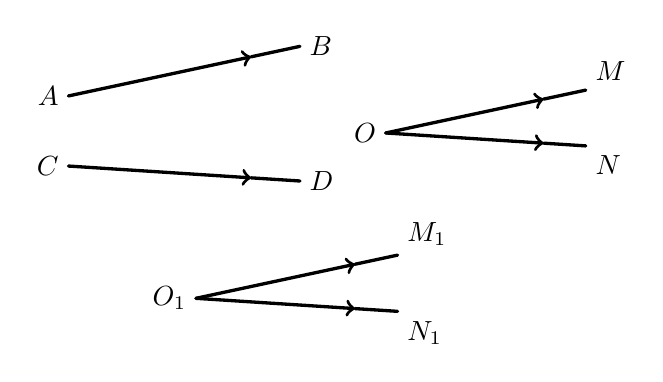
\begin{tikzpicture}[line cap=round,line join=round]
    \coordinate (A) at (-3.55,1.29);
    \coordinate (B) at (-0.61,1.92);
    \coordinate (C) at (-3.55,0.40);
    \coordinate (D) at (-0.61,0.21);
    \coordinate (O) at (0.48,0.82);
    \coordinate (M) at (3.02,1.3643);
    \coordinate (N) at (3.02,0.6559);
    \coordinate (O1) at (-1.93,-1.28);
    \coordinate (M1) at (0.63,-0.7314);
    \coordinate (N1) at (0.63,-1.4454);

    \foreach \first/\last in {A/B,C/D,O/M,O/N,O1/M1,O1/N1}{
        \path (\first) -- (\last) coordinate[pos=0.79] (arrow);
        \draw[very thick,->] (\first) -- (arrow);
        \draw[very thick] (arrow) -- (\last);
    }
    \node[left] at (A) {\(A\)};
    \node[right] at (B) {\(B\)};
    \node[left] at (C) {\(C\)};
    \node[right] at (D) {\(D\)};
    \node[left] at (O) {\(O\)};
    \node[above right] at (M) {\(M\)};
    \node[below right] at (N) {\(N\)};
    \node[left] at (O1) {\(O_1\)};
    \node[above right] at (M1) {\(M_1\)};
    \node[below right] at (N1) {\(N_1\)};
\end{tikzpicture}

    \caption{Угол \(MON\) двух скрещивающихся прямых \(AB\) и \(CD\)}\label{fig:kiselev-stereo-340}
\end{figure}

Величина угла \(MON\) не зависит от положения точки \(O\). В самом деле, если построим указанным способом угол \(M_1O_1N_1\) при какой-нибудь другой точке \(O_1\), то \(MON=M_1O_1N_1\), так как эти углы имеют соответственно параллельные и одинаково направленные стороны (\hyperref[para:lines-parallel-to-same-line]{см.~§~\ref*{para:lines-parallel-to-same-line}} и \hyperref[para:angles-with-parallel-sides]{§~\ref*{para:angles-with-parallel-sides}}).

\section*{Угол, образуемый прямой с плоскостью}
\addcontentsline{toc}{section}{Угол, образуемый прямой с плоскостью}

\kiselevparagraph{para:orthogonal-projection-on-plane} \textbf{Проекция прямой на плоскость.} Мы говорили прежде (\hyperref[para:normal-and-oblique-lengths]{см.~§~\ref*{para:normal-and-oblique-lengths}}), что, когда из одной точки проведены к плоскости перпендикуляр и наклонная, то проекцией этой наклонной на плоскость называется прямая, соединяющая основание
% Печатная с. 299.
перпендикуляра с основанием наклонной. Дадим теперь более общее определение проекции.

\begin{enumerate}[label=\arabic*),ref=\arabic*]
    \item \emph{Проекцией какой-нибудь точки на плоскость} (например, точки \(M\) на плоскость \(P\), рис.~\ref{fig:kiselev-stereo-341}) называется \emph{основание} \(m\) \emph{перпендикуляра, опущенного на эту плоскость из взятой точки}.
    \item \emph{Проекцией какой-нибудь линии на плоскость} называется \emph{геометрическое место проекций всех точек этой линии}.
\end{enumerate}

\begin{figure}[htbp]
    \centering
    \renewcommand{\thefigure}{341}
    \captionsetup{name=Рис.,labelsep=period}
    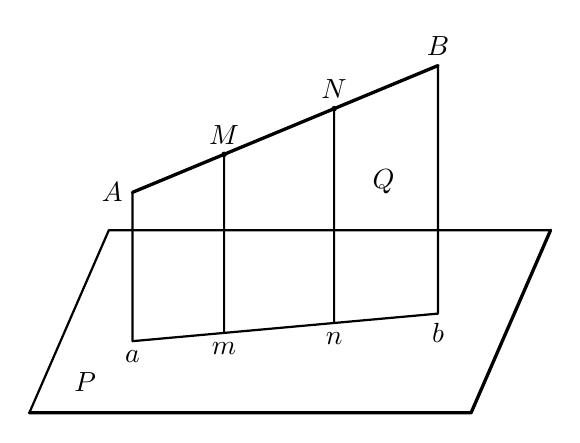
\begin{tikzpicture}[line cap=round,line join=round]
    \coordinate (A) at (-2.00,1.35);
    \coordinate (B) at (1.88,2.96);
    \coordinate (a) at (-2.00,-0.54);
    \coordinate (b) at (1.88,-0.19);
    \path (A) -- (B) coordinate[pos=0.30] (M) coordinate[pos=0.66] (N);
    \path (a) -- (b) coordinate[pos=0.30] (m) coordinate[pos=0.66] (n);
    \draw[thick] (-3.31,-1.45) -- (-2.30,0.87) -- (3.31,0.87);
    \draw[very thick] (-3.31,-1.45) -- (2.30,-1.45) -- (3.31,0.87);
    \draw[thick] (a) -- (A) (m) -- (M) (n) -- (N) (b) -- (B) (a) -- (b);
    \draw[very thick] (A) -- (B);
    \foreach \point in {M,N} {
        \fill (\point) circle[radius=1pt];
    }
    \node[left] at (A) {\(A\)};
    \node[above] at (B) {\(B\)};
    \node[above] at (M) {\(M\)};
    \node[above] at (N) {\(N\)};
    \foreach \point in {a,m,n,b} {
        \node[below] at (\point) {\(\point\)};
    }
    \node at (-2.60,-1.06) {\(P\)};
    \node at (1.19,1.48) {\(Q\)};
\end{tikzpicture}

    \caption{Проекции точек \(A\), \(M\), \(N\), \(B\) прямой \(AB\) на плоскость \(P\)}\label{fig:kiselev-stereo-341}
\end{figure}

В частности, если проецируемая линия --- \emph{прямая} (например, \(AB\), рис.~\ref{fig:kiselev-stereo-341}), то её проекция на плоскость \(P\) --- также \emph{прямая}. В самом деле, если через прямую \(AB\) и перпендикуляр \(Mm\), опущенный на плоскость проекций из какой-нибудь одной точки \(M\) этой прямой, проведём плоскость \(Q\), то эта плоскость должна быть перпендикулярна к плоскости \(P\) (\hyperref[para:perpendicular-planes-criterion]{см.~§~\ref*{para:perpendicular-planes-criterion}}). Поэтому перпендикуляр, опущенный на плоскость \(P\) из любой точки прямой \(AB\) (например, из точки \(N\)), должен лежать в этой плоскости \(Q\) (\hyperref[para:normal-in-perpendicular-plane]{см.~§~\ref*{para:normal-in-perpendicular-plane}}). Следовательно, проекции всех точек прямой \(AB\) должны лежать на прямой \(ab\), по которой пересекаются плоскости \(P\) и \(Q\). Таким образом, эта прямая \(ab\) представляет собой геометрическое место проекций всех точек данной прямой \(AB\) и, следовательно, является её проекцией.

Существует, впрочем, один частный случай, когда \emph{проекция прямой становится точкой}. Это бывает тогда, когда прямая перпендикулярна к плоскости проекций.

\kiselevparagraph{para:angle-between-line-and-plane} \textbf{Угол прямой с плоскостью.} \emph{Углом прямой} \(AB\) (рис.~\ref{fig:kiselev-stereo-342}) \emph{с плоскостью} \(P\) в том случае, когда прямая наклонна к плоскости, называется \emph{угол} \(ABC\)\emph{, образованный этой прямой и её проекцией на плоскость}.

\begin{figure}[htbp]
    \centering
    \renewcommand{\thefigure}{342}
    \captionsetup{name=Рис.,labelsep=period}
    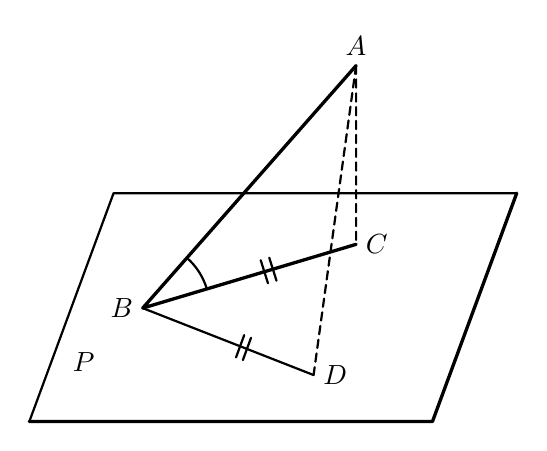
\begin{tikzpicture}[line cap=round,line join=round]
    \coordinate (A) at (1.1,2.9);
    \coordinate (B) at (-1.61,-0.18);
    \coordinate (C) at (1.1,0.63);
    \coordinate (D) at (0.56,-1.03);
    \draw[thick] (-3.05,-1.62) -- (-1.98,1.28) -- (3.14,1.28);
    \draw[very thick] (-3.05,-1.62) -- (2.07,-1.62) -- (3.14,1.28);
    \draw[thick,densely dashed] (A) -- (C) (A) -- (D);
    \draw[very thick] (A) -- (B) -- (C);
    \draw[thick] (B) -- (D);
    \draw[thick] (B) ++(16.64:0.85) arc[start angle=16.64,end angle=48.65,radius=0.85];
    \path (B) -- (C) coordinate[pos=0.57] (CtickA) coordinate[pos=0.61] (CtickB);
    \path (B) -- (D) coordinate[pos=0.57] (DtickA) coordinate[pos=0.61] (DtickB);
    \draw[thick] (CtickA) ++(0.046,-0.146) -- ++(-0.092,0.292)
        (CtickB) ++(0.046,-0.146) -- ++(-0.092,0.292)
        (DtickA) ++(-0.052,-0.142) -- ++(0.104,0.284)
        (DtickB) ++(-0.052,-0.142) -- ++(0.104,0.284);
    \node[above] at (A) {\(A\)};
    \node[left] at (B) {\(B\)};
    \node[right] at (C) {\(C\)};
    \node[right] at (D) {\(D\)};
    \node at (-2.36,-0.87) {\(P\)};
\end{tikzpicture}

    \caption{Угол \(ABC\), образованный наклонной \(AB\) и её проекцией \(BC\)}\label{fig:kiselev-stereo-342}
\end{figure}

% Печатная с. 300.
Этот угол обладает тем свойством, что он \emph{наименьший} из всех углов, которые наклонная образует с прямыми, проведёнными в плоскости \(P\) через основание наклонной. Докажем, например, что \(\angle ABC\) меньше \(\angle ABD\). Для этого отложим \(BD=BC\) и соединим \(D\) с \(A\). У треугольников \(ABC\) и \(ABD\) две стороны одного равны соответственно двум сторонам другого, но третьи стороны не равны, а именно \(AD>AC\) (\hyperref[para:normal-and-oblique-lengths]{см.~§~\ref*{para:normal-and-oblique-lengths}}). Вследствие этого \(\angle ABD\) больше \(\angle ABC\) (\kiselevPlanimetryPage{51}{см.~Планиметрия, §~58, пункт~2}).

\clearpage
\endgroup
